\documentclass{standalone}
\usepackage{tikz}
\begin{document}
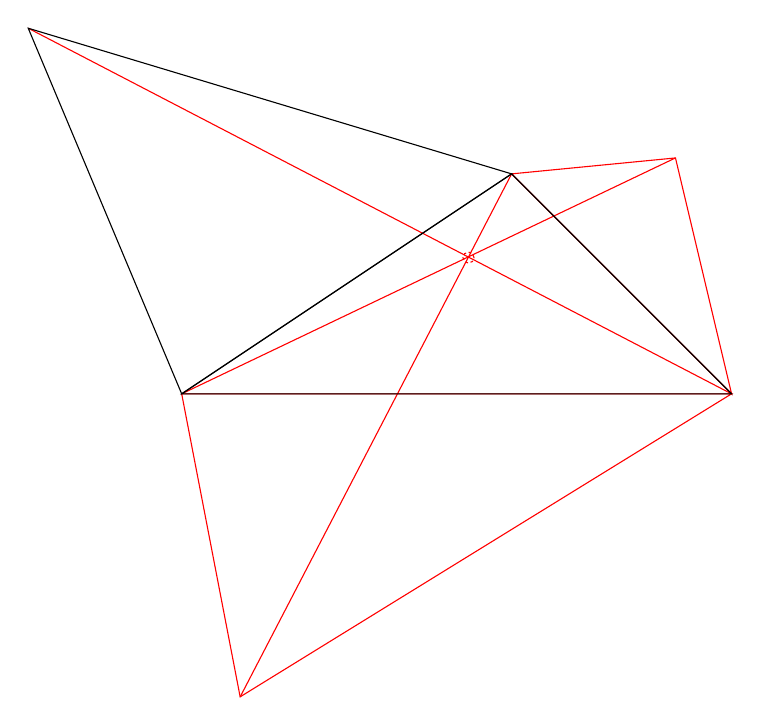
\begin{tikzpicture}[x=1pt,y=1pt]
\draw[red] (75.51,-152.95) -- (96.64,-262.44) -- (274.21,-152.95) -- cycle;
\draw[red] (194.73,-73.47) -- (253.94,-67.71) -- (274.21,-152.95) -- cycle;
\draw[red] (194.73,-73.47) -- (96.65,-262.44);
\draw[red] (20.06,-20.84) -- (274.21,-152.96);
\draw[red] (75.51,-152.95) -- (253.93,-67.71);
\draw[red, dash pattern=on 1pt] (179.15,-103.72) circle (2.00);
\draw (75.51,-152.95) -- (274.21,-152.95) -- (194.73,-73.47) -- cycle;
\draw (75.51,-152.95) -- (20.06,-20.84) -- (194.73,-73.47) -- cycle;
\end{tikzpicture}
\end{document}
